% Two-page anonymous review draft, styled after the supplied UAV draft.
% Confirm against the current CVIS 2026 Overleaf template before submission.
\documentclass[letterpaper,10pt,twocolumn]{article}
\usepackage[T1]{fontenc}
\usepackage{times}
\usepackage[left=0.8in,right=0.8in,top=0.8in,bottom=0.8in,columnsep=0.3in]{geometry}
\usepackage{amsmath,amssymb,booktabs,graphicx}
\usepackage{tikz}
\usetikzlibrary{arrows.meta,positioning}
\usepackage{caption}
\usepackage{balance}
\captionsetup{font=small,labelfont=bf}
\usepackage[hidelinks,pdfauthor={},pdftitle={PJSS: Sparse Equation Discovery from a Noisy Trajectory}]{hyperref}
\setlength{\parindent}{1em}
\setlength{\parskip}{0pt}
\setlength{\textfloatsep}{10pt}
\setlength{\floatsep}{8pt}
\setlength{\abovecaptionskip}{5pt}
\setlength{\belowcaptionskip}{0pt}
\newcommand{\lead}[1]{\par\smallskip\noindent\textbf{#1}\ }
\makeatletter
\renewcommand\section{\@startsection{section}{1}{\z@}{-2.5ex plus -0.8ex minus -0.2ex}{1.1ex plus 0.2ex}{\normalfont\large\bfseries}}
\renewcommand\@seccntformat[1]{\csname the#1\endcsname.\quad}
\makeatother
\begin{document}
\twocolumn[{\centering\vspace*{0.35in}
{\large\bfseries PJSS: Sparse Equation Discovery from a Noisy Trajectory\par}
\vspace{0.20in}}]

\begin{center}\textbf{\large Abstract}\end{center}
\noindent\textit{We study recovery of sparse differential equations from one noisy trajectory. Profiled Joint Subset Search (PJSS) alternates joint estimation of states and coefficients with a search for better combinations of equation terms. A local quadratic model accounts for how the estimated trajectory can change, allowing many supports to be screened before nonlinear refitting. Sparsity is selected using a BIC-inspired score with fixed development-selected defaults. Across 77 in-library chaotic systems, PJSS recovers the exact terms in 89.0\% of runs, including 85.3\% on 49 systems outside development benchmarks. On 64 paired runs from 35 new systems, it recovers 53, compared with 36 or 41 for DEDi under two selection rules. Ablations show that subset proposals supply the larger gain, with a smaller additional benefit from profiling. These results concern simulated, fully observed systems; measured-data tests expose failures.}

\section{The task and method}
We observe a uniformly sampled trajectory corrupted by measurement noise and seek a sparse ordinary differential equation,
\begin{equation}
 y_i=x(i\Delta t)+e_i,\qquad \dot x=C^\top\theta(x).
\end{equation}
Here $\theta$ is a supplied library of candidate functions and the nonzero entries of $C$ identify the terms in each equation. The default three-dimensional library contains the 20 monomials of degree at most three. The sampling interval and library are inputs; neither the true noise level nor the number of terms is supplied.

Sparse identification methods such as SINDy~\cite{sindy} select terms by regression. Weak formulations~\cite{weak} reduce the need to differentiate noisy measurements, while joint methods such as SIDDS~\cite{sidds} and DEDi~\cite{dedi} estimate the trajectory and equations together. Joint fitting can be expensive when many supports must be tried. PJSS uses a cheap proposal step to decide which supports deserve that fit.

\lead{Joint fitting.} For a fixed support, PJSS estimates denoised states and active coefficients together. Its objective combines a robust observation loss with a soft midpoint-rule dynamics constraint. A banded state matrix and a small coefficient border make each solver iteration linear in record length for fixed dimension and library size.

\lead{Proposing terms.} At the current fit, PJSS forms a quadratic approximation over all library coefficients, including inactive terms. Eliminating state increments gives a \emph{profiled} quadratic: a coefficient change is assessed while allowing local adjustment of the trajectory. The search then ranks subsets of up to five terms per equation. For the default library this enumerates 21,699 nonempty subsets per equation; larger libraries use beam search.

\begin{figure}[t]
\centering
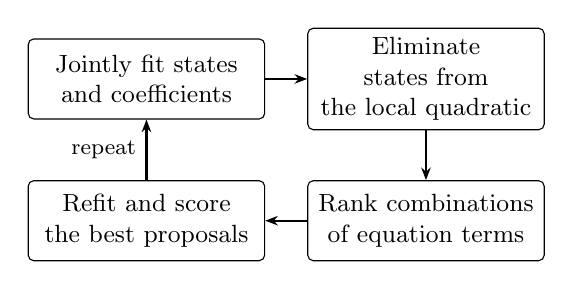
\begin{tikzpicture}[
 box/.style={draw,rounded corners=2pt,align=center,text width=1.09in,minimum height=0.40in,font=\small},
 arr/.style={-{Stealth[length=1.6mm]},thick}]
\node[box] (fit) at (0,0) {Jointly fit states\\and coefficients};
\node[box] (profile) at (3.55,0) {Eliminate states from\\the local quadratic};
\node[box] (search) at (3.55,-1.8) {Rank combinations\\of equation terms};
\node[box] (refit) at (0,-1.8) {Refit and score\\the best proposals};
\draw[arr] (fit)--(profile);
\draw[arr] (profile)--(search);
\draw[arr] (search)--(refit);
\draw[arr] (refit)--node[left,font=\footnotesize]{repeat}(fit);
\end{tikzpicture}
\caption{PJSS screens many candidate supports with a local quadratic and reserves nonlinear joint fits for the most promising. The combined search is not globally exhaustive.}
\label{fig:method}
\end{figure}

\lead{Refitting and selection.} The best proposals undergo nonlinear joint refitting; a BIC-inspired score compares their observation and dynamics errors with a complexity penalty. Residual-based noise calibration and autocorrelation corrections help prevent overfitting. An AR(1) observation model is selected automatically for strongly correlated noise in three dimensions. Defaults are fixed from development data. Cheap truth-free methods provide starting supports, and two proposal rounds are used by default (Figure~\ref{fig:method}).

\section{What we tested}
\lead{Recovery across systems.} The external \texttt{dysts} benchmark~\cite{dysts} contains 77 systems representable in our libraries: 61 three-dimensional systems and 16 of dimension 4--6. We evaluate 6,160 simulated trajectories, using 500 or 2,000 samples and measurement noise of 1--20\% of each coordinate's standard deviation. Forty-nine systems lie outside our development benchmarks; the others overlap or share a support with them. Exact recovery requires the correct nonzero pattern in every equation.

\lead{Comparison with joint discovery.} We compare with the authors' DEDi code using its full 35-setting grid. One paired study samples 80 runs from five conditions on development-system families: white, coloured and heavy-tailed noise, short records, and a high-noise stress condition. A second uses 64 runs from 35 new three-dimensional \texttt{dysts} systems. DEDi selects its model by validation error or BIC. Protocols were recorded in the repository before these comparisons.

\lead{Separating the components.} Ablations use 576 runs drawn from white noise, coloured noise, a high-noise stress set and three-dimensional \texttt{dysts}. They remove subset proposals, replace enumeration with forward stepwise selection, or form proposals with states fixed. The last variant retains subset enumeration and nonlinear joint refits, isolating the contribution of profiling.

\clearpage
\section{What the tests showed}
\balance
\lead{Broad recovery within the library.} PJSS recovers exact support in 89.0\% of the 6,160 \texttt{dysts} runs and 85.3\% on the 49 new systems. These rates measure recovery under simulated measurement noise with a library that contains the generating equations.

\begin{table}[t]
\centering
\caption{Exact support recovery in paired full-grid comparisons. Each entry is a count of recovered runs; the two studies use different system sets.}
\label{tab:dedi}
\small
\begin{tabular}{@{}lrr@{}}
\toprule
Method / selection & Core systems & New systems\\
 & ($n=80$) & ($n=64$)\\
\midrule
\textbf{PJSS} & \textbf{66} & \textbf{53}\\
DEDi / validation & 55 & 36\\
DEDi / BIC & 61 & 41\\
\bottomrule
\end{tabular}
\end{table}

\lead{The DEDi advantage depends on the setting.} Table~\ref{tab:dedi} shows the paired comparisons. On the core-system study, the 66 versus 61 comparison does not establish superiority over DEDi-BIC; excluding coloured noise, both recover 56/64. On new systems, PJSS recovers 53/64 against 41/64 for DEDi-BIC, with 15 paired wins and three losses. The gain is concentrated at 1--5\% noise (29/32 versus 19/32); at 10--20\% noise the counts are 24/32 and 22/32. A post-hoc system bootstrap gives a 95\% interval of 4.4--34.4 percentage points for PJSS minus DEDi-BIC.

\lead{Subset proposals supply the larger gain.} Removing proposals loses 32 exact recoveries and gains none; replacing enumeration with forward stepwise selection loses 28 and gains none. In the separate profiling comparison, PJSS recovers 490/576 runs versus 480/576 with fixed-state proposals, with 15 paired wins and five losses. Profiling helps, but its extra benefit is smaller and varies by setting.

\section{What this means and where it fails}
PJSS makes support search inside joint equation discovery more tractable: many term combinations are screened without repeatedly solving the full nonlinear estimation problem. The contribution is the coupling of subset proposals and joint refits; joint estimation, state elimination and quadratic screening are established ingredients. Profiled smoothing approximations have also been used for ODE model selection~\cite{zhang}.

The search has no global-optimality guarantee. Candidate supports are limited in size, larger libraries use approximate search, and constants were chosen during development. Some test archives informed later revisions, which were subsequently checked on fresh archives; the evidence should not be described as one untouched test throughout development. The paired comparison uses the current version, while the broad benchmark rate comes from an earlier frozen version; its reported change on that benchmark is 0.1 percentage point.

Measured-data results do not establish practical reliability. On a single pendulum, the selected support fails the prescribed criterion, although dependent library terms make support interpretation ambiguous. On a double pendulum, whose rational dynamics lie outside the library, forecasts are worse than SINDy baselines and the ambiguity flag remains silent. Process noise, irregular sampling and general library misspecification remain unvalidated. The present evidence supports sparse equation recovery for fully observed, in-library simulated dynamics.

\begin{thebibliography}{6}
\small
\bibitem{sindy} S.~L. Brunton, J.~L. Proctor, and J.~N. Kutz. Discovering governing equations from data by sparse identification of nonlinear dynamical systems. \emph{PNAS}, 113:3932--3937, 2016.
\bibitem{weak} D.~A. Messenger and D.~M. Bortz. Weak SINDy: Galerkin-based data-driven model selection. \emph{Multiscale Modeling \& Simulation}, 19:1474--1497, 2021.
\bibitem{sidds} J.~M. Hokanson, G.~Iaccarino, and A.~Doostan. Simultaneous identification and denoising of dynamical systems. \emph{SIAM J. Scientific Computing}, 45:A1413--A1437, 2023.
\bibitem{dedi} T.~Meissner and K.~Glasner. Simultaneous model discovery and state estimation under high data corruption. \emph{SIAM J. Applied Dynamical Systems}, 25:1439--1467, 2026.
\bibitem{dysts} W.~Gilpin. Chaos as an interpretable benchmark for forecasting and data-driven modelling. \emph{NeurIPS Datasets and Benchmarks}, 2021.
\bibitem{zhang} X.~Zhang, J.~Cao, and R.~J. Carroll. On the selection of ordinary differential equation models with application to predator-prey dynamical models. \emph{Biometrics}, 71:131--138, 2015.
\end{thebibliography}
\end{document}
